%%% LyX 2.0.5.1 created this file.  For more info, see http://www.lyx.org/.
%%% Do not edit unless you really know what you are doing.
%\documentclass[12pt,english]{report}
%\usepackage{mathptmx}
%\renewcommand{\familydefault}{\rmdefault}
%\usepackage[T1]{fontenc}
%\usepackage[latin9]{inputenc}
%\usepackage[a4paper]{geometry}
%\setcounter{secnumdepth}{2} % Changed from 3 to 2. 0-chapter 1-section 2-subsection 
%\setcounter{tocdepth}{2} % Changed from 3 to 2. 0-chapter 1-section 2-subsection 
%\setlength{\parskip}{\medskipamount}
%\setlength{\parindent}{0pt}
%\usepackage{verbatim}
%\usepackage{pdfpages}
%\usepackage{graphicx}
%\usepackage{subfig} %% This package has to be here
%\usepackage{setspace}
%\usepackage{arabtex}
%\usepackage[numbers]{natbib}
%\usepackage{nomencl}
%\usepackage{paralist}
%\usepackage{amsthm}
%\usepackage{amsmath}
%\usepackage{amsfonts}
%\usepackage{etoolbox}
%\newtoggle{edit-mode}
%\togglefalse{edit-mode}  
%\toggletrue{edit-mode}
%\iftoggle{edit-mode}{
%\geometry{verbose,tmargin=2cm,bmargin=2cm,lmargin=2cm,rmargin=6cm,headheight=1cm,headsep=1cm,footskip=1cm, marginparwidth=5cm}
%}{
%\geometry{verbose,tmargin=2cm,bmargin=2cm,lmargin=2cm,rmargin=2cm,headheight=1cm,headsep=1cm,footskip=1cm}
%}
%
%\makenomenclature
%
%% Theorem Styles
%\newtheorem{theorem}{Theorem}[section]
%% Definition Styles
%%\theoremstyle{definition}
%\newtheorem{definition}{Definition}[section]
%\newtheorem{example}{Example}[section]
%\theoremstyle{remark}
%\newtheorem{remark}{Remark}
%
%\usepackage[linesnumbered]{algorithm2e}
%
%\begin{document}

\chapter{Ongoing Strokes Segmentation}
\label{chap:segmentation}

\emph{see: \cite{al2010development} for Arabic script segmentation problem}
  
\section{The Proposed Segmentation Approach}
\label{sec:approach}

\textbf{Complexity measure:} this value indicates the curvature degree of a given 2-D trajectory $T=\{p_i\}_{i=1}^{n}$. 
Preprocessing steps, which include simplification and re-sampling, are required to ensure invariance under scaling and data imperfections. 
The complexity measure is calculated by summing the parameters $\alpha_{k}$ computed for each inner point $p_k$ in $T$ for $2 \leq k \leq n-1$, i.e., $CM(T)=\sum_{k=2}^{n-1}{\alpha_k}$.
The parameter $\alpha_{k}$ is defined as:
\begin{equation}
\alpha_{k}=\frac{\pi-\phi_{k}}{\frac{\pi}{6}}
\end{equation}
where $\phi_k=\angle(\overline{p_{k-1}p_{k}},\overline{p_{k}p_{k+1}})$.

The proposed approach goes through three stages. 
In the first stage, \emph{points of interest} (POIs), are continuously nominated while the stroke is being scribed.
The sub-strokes imposed by these POIs are scored by an Arabic letter classifier. 
In the second stage, once the entire stroke is available, a rules-based process is used to refine the set of POIs and re-score the sub-strokes. 
Eventually, the system heuristically determines the final set of SPs based on the sub-strokes scoring. See Figure \ref{fig:system_flow}. 

\begin{figure}
\centering
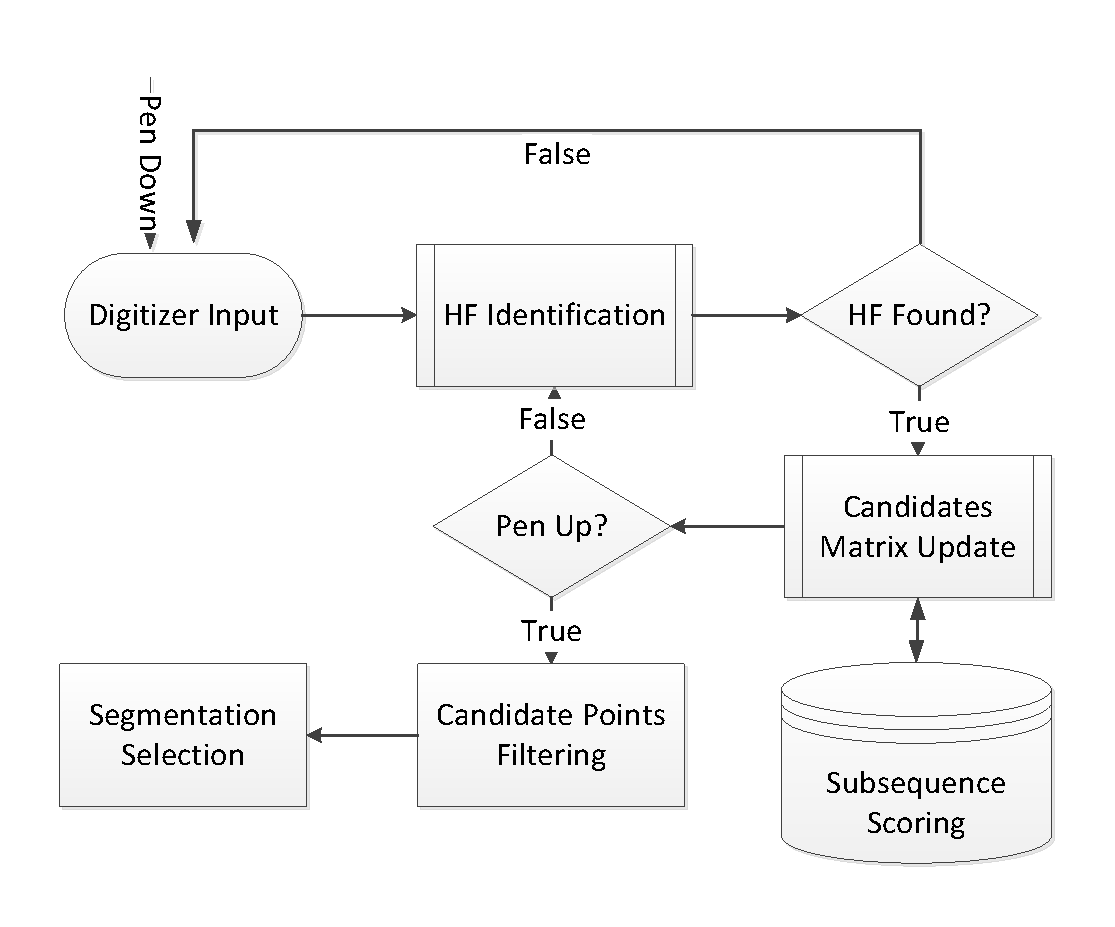
\includegraphics[width=0.8\textwidth]{./figures/system_flow}
\caption{High level visualization of the system flow.}
\label{fig:system_flow}
\end{figure}

\subsection{First Stage: POIs Nomination and Sub-strokes Scoring}

\textbf{Horizontal fragment identification:} in this stage, the system attempts to identify \emph{horizontal fragments} (HFs) that join pairs of connected letters. 
These handlers are horizontal, directed right to left and located near the baseline (see Figure  \ref{fig:horizontal_fragments}). 
Using a smoothed version of the trajectory helps the process to ignore undesired small horizontal regions that are frequently caused by the digitizer's imperfection.  
A point $p_{i}$ is defined as a "horizontal point" if the slope of the line $\overline{p_{i-1}p_{i}}$ is less than a preset value $\delta$, which was empirically tuned to $0.6$. The same exact value for this parameter was found independently in \cite{daifallah2009recognition}.

\begin{figure}
\centering
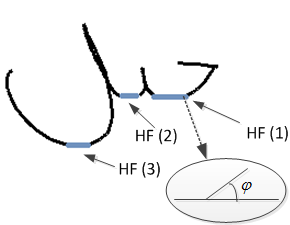
\includegraphics[width=0.4\columnwidth]{./figures/horizontal_fragments}
\caption{Horizontal Fragments [HF] of the word \RL{jbl} (JABAL).}
\label{fig:horizontal_fragments}
\end{figure}

HFs are continuously identified using the following process.
The first detected horizontal point is set as an "HF starting point". 
All the subsequent horizontal points are ignored until a non-horizontal point is detected, indicating the end of an HF sequence. 
This point is identified as an "HF ending point" and the medial point of an HF is marked as POI. 
POIs are potential SPs, thus, this process yields an over-segmentation of the stroke. 
While false positive SPs can be easily removed, missed real SPs cannot be easily recovered. 
Therefore, in order to minimize the miss-rate, this process is delicate and allows false HFs to be detected.

In a post processing step, fractions of the same horizontal segment, which were identified as multiple HFs, are rejoined to a single HF. 
The merging is done by evaluating the complexity measurement across the two consequent HFs, see Figure \ref{fig:candidate_in_no_horizontal}.

\begin{figure}
\centering
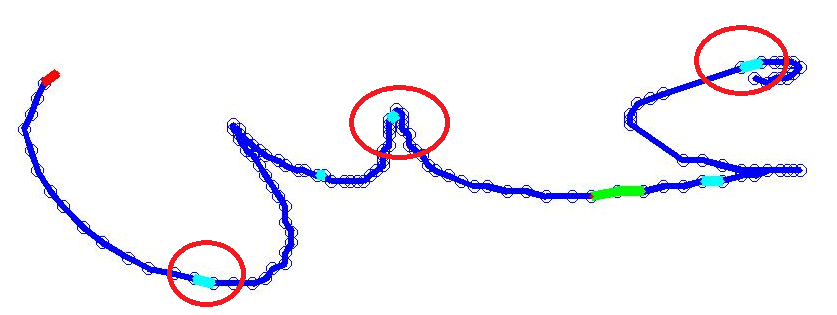
\includegraphics[width=0.4\textwidth]{./figures/candidate_in_no_horizontal}
\caption{The main body of Arabic word \RL{`yn} (AIN). POIs are colored in cyan. The green areas indicate merge between two subsequent HFs. Three types of false POIs can be seen: 1. A POI at the beginning of a stroke. 2. A POI that is caused by a bad HF. 3. A POI that resides in a letter's valley. }
\label{fig:candidate_in_no_horizontal}
\end{figure}

\textbf{Sub-strokes scoring:}
Let $S=\{p_{i}\}_{i=1}^{n}$ be a sequence representing a handwritten stroke in which $L$ POIs were detected. 
Let $KP=\{KP_{i}\}_{i=0}^{L+1}$ (Key points) be the ordered set of POIs, in addition to the first and the last points of the stroke positioned as the first and the last items in the set.
Formally, we define: 
\begin{equation}
KP_{i} =\begin{cases}    1		, & \mbox{if } i=0 \\
							   POI_{i}	, & \mbox{if } 1\leq i \leq L \\
							   n    , & \mbox{if } i=L+1 
			\end{cases}				
\end{equation}
A sub-stroke $S_{i}^{j}$ is a sub-sequence of the stroke $S$ that starts at $KP_{i}$ and ends at $KP_{j}$, formally:
\begin{equation}
S_{i}^{j}=\{p_{k}\}_{k=KP_{i}}^{KP_{j}}; i<j
\end{equation}

We generate an upper triangular scoring matrix $D\in\mathbb{R}^{(L+1)\times (L+1)}$ where each cell $D_{i,j}$ represents the sub-stroke $S_i^j$. It contains the information returned by the scoring system for the sub-strokes $S_i^j$. 
The matrix $D$ is generated dynamically; adding a row and a column for each new detected POI. 
Imposing a locality constraint which narrows the band of the $D$ matrix above the main diagonal improved the efficiency of the process and the segmentation accuracy. 
Given a band width $B$ we fix $D_{i,j}=\infty$ if  $j \leq i$ or $j-i>B$.
We argue that sub-strokes representing a letter will achieve, in most cases, better scoring, i.e., lower $D_{i,j}$ value than other sub-strokes.

\begin{figure}
\centering
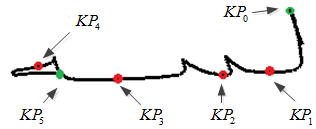
\includegraphics[width=0.5\textwidth]{./figures/candidate_points}
\caption{KPs of the word \RL{lbyh} (Lbyh). POIs are colored in red. The first and last key points (KPs) are colored in green. }
\label{fig:candidate_points}
\end{figure}

The classifier contains four databases, one for each letter position. 
It receives a sequence of points, which represent the sub-stroke, and a letter position (Ini, Mid, Fin and Iso), and returns a list of the nearest neighbors and their scoring. 
This scoring indicates the similarity measure between the sequence and the candidate.
The relative location of the sub-stroke was used to avoid accessing all the four databases. 
As can be seen in Table \ref{table:subsequences_types}, we differentiate between four types of subsequences. 
For each type, we indicate the set of databases that need to be examined, i.e., the possible letter positions the sub-stroke may represent. 
In Table \ref{table:subsequences_types}, $S$ denotes a stroke containing $L$ POIs where $m>0$ and $k<L+1$.

\begin{table}
\centering
\renewcommand{\arraystretch}{1.3}
\caption{A mapping between the subsequence types and the possible letter positions}
\begin{tabular}{| c |c | c |}
\hline
  Name     & Subsequence    & Letter Position    \\
\hline
  $\alpha$ & $S_0^{k}$         & $Ini$ or $Mid$  \\
\hline
  $\beta$  & $S_{m}^{k}$     & $Mid$              \\
\hline
  $\chi$    & $S_{m}^{L+1}$ & $Mid$ or $Fin$   \\
\hline
  $\delta$ & $S_0^{L+1}$     & All                   \\
\hline
\end{tabular}
\label{table:subsequences_types}
\end{table}

The relation between the cells in the matrix $D$ and the sub-stroke type is given in matrix $D_p$  (Equation \ref{eq:positions_matrix}). 
The type of the sub-stroke can be determined while the stroke is being scribed.
The last column and row are added on the "pen up" event.


\begin{equation}
D_{p}=
\left( 
\begin{array}{ccccccc}
\infty 	& \alpha & \alpha & \alpha  & \cdots & \alpha & \delta \\
\infty  & \infty  & \beta   & \beta   & \cdots  & \beta  & \chi    \\
\infty  & \infty  & \infty   & \beta   & \cdots  & \beta  & \chi    \\
\vdots & \vdots & \vdots  & \vdots & \ddots  & \vdots & \vdots \\
\infty  & \infty  & \infty   & \infty   & \cdots  & \beta  & \chi    \\
\infty  & \infty  & \infty   & \infty   & \cdots  & \infty  & \chi    \\
\infty  & \infty  & \infty   & \infty   & \cdots  & \infty  & \infty \end{array} \right)
\label{eq:positions_matrix}
\end{equation}\\

For a given input (sequence and position), the recognition system returns the $K$ nearest neighbors with different labeling, where the labeling is defined as the tuple (letter, position). In our implementation, we set $K=3$.

\begin{figure}
\centering
\renewcommand{\arraystretch}{1.1}
\begin{tabular}{| c |c | c | c| c | c | c |}
\hline
     & $0$ & $1$ & $2$ & $3$ & $4$ & $5$\\
\hline
$0$
   & N/A
   & \subfloat{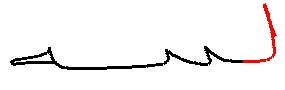
\includegraphics[width=1.8cm]{./figures/substrokes/L}}
   & \subfloat{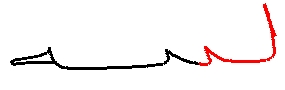
\includegraphics[width=1.8cm]{./figures/substrokes/LB1}}
   & \subfloat{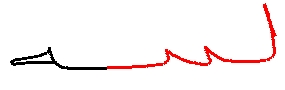
\includegraphics[width=1.8cm]{./figures/substrokes/LB1B2}}
   & N/A & N/A \\
\hline
$1$
   & N/A & N/A
   & \subfloat{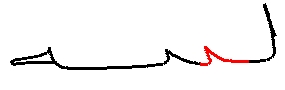
\includegraphics[width=1.8cm]{./figures/substrokes/B1}}
   & \subfloat{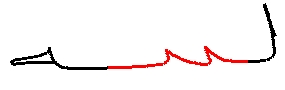
\includegraphics[width=1.8cm]{./figures/substrokes/B1B2}}
   & \subfloat{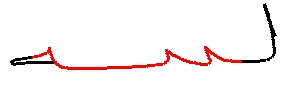
\includegraphics[width=1.8cm]{./figures/substrokes/B1B2H1}}
   & N/A \\
\hline
$2$
   & N/A  & N/A & N/A
   & \subfloat{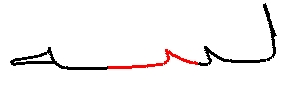
\includegraphics[width=1.8cm]{./figures/substrokes/B2}}
   & \subfloat{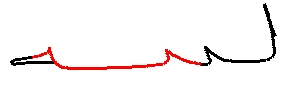
\includegraphics[width=1.8cm]{./figures/substrokes/B2H1}}
   & \subfloat{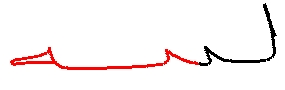
\includegraphics[width=1.8cm]{./figures/substrokes/B2H}} \\
\hline
$3$
   & N/A & N/A & N/A & N/A
   & \subfloat{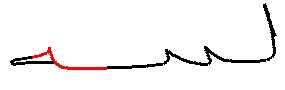
\includegraphics[width=1.8cm]{./figures/substrokes/H1}}
   & \subfloat{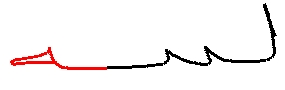
\includegraphics[width=1.8cm]{./figures/substrokes/H}} \\
\hline
$4$
   & N/A & N/A & N/A & N/A & N/A
   & \subfloat{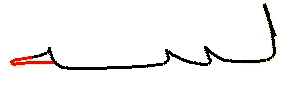
\includegraphics[width=1.8cm]{./figures/substrokes/H2}}\\
\hline
$5$
   & N/A & N/A & N/A & N/A & N/A & N/A \\
\hline
\end{tabular}
\caption{A tabular representation of the $D$ matrix that corresponds the KPs showed in Figure \ref{fig:candidate_points}. Each cell visually demonstrates the matching sub-stroke colored in red.}
\label{table:substrokes_demo} 
\end{figure}

\subsection{Second Stage: Candidate points filtering and scoring correction}
In this stage we re-score subsequences and eliminate redundant POIs based on the following rules:\\

\begin{compactitem}
	\item Inner SPs should lie close to the baseline. 
	\item SPs do not reside in loops.
	\item The sub-stroke length should be proportional to the length of the containing stroke.
\end{compactitem}

\textbf{Baseline detection:} The system determines the baseline by calculating the vertical density histogram of the re-sampled and normalized sub-stroke. 
The height of the stroke (y-axis) is partitioned into ten equi-length intervals. 
A POI is filtered out if it does not satisfy the following condition:
\begin{equation}
|POI_y-I_{max}| \leq 2*max{({|I|},0.15)} 
\end{equation}
where $POI_y$ represents the $y$-coordinate of the POI; $|I|$ is the length of an interval; and $I_{max}$ denotes the center of the most inhabited interval. 
In order to reliably determine the baseline, the baseline detection algorithm is activated only after the fourth POI is detected. 
This process has proven to be very effective in eliminating challenging false POIs that reside in valleys of frequently used final Arabic letters, such as \RL{-q}, \RL{-s} and \RL{-n}. 
An example of such a POI can be seen in the letter \RL{-n} in Figure \ref{fig:candidate_in_no_horizontal}. 
The baseline is needed only to verify that the POIs are in a reasonable distance from it, therefore, imprecise valuation of the position or the direction of the baseline is tolerable.

The third rule is used to penalize unreasonably low scoring given to small sub-strokes, which are unlikely to represent a letter. 
This is done by calculating the ratio of the sub-stroke length proportional to the entire stroke length.
For instance, it is common to add a small, hook-like, extension to the suffix of the letter \RL{d}. 
This extension may look very similar to the letter \RL{-a} during the stroke scribing; and thus under-scored by the recognition system, and eventually, result in over-segmenting the letter \RL{d}. In some cases, POIs are incorrectly nominated on non-horizontal areas. This is caused due to noises in the data and the fact that the nomination is done while the word is being scribed. Our filtering algorithm should be corrected, in a future work, to handle this case.

\subsection{Third Stage: Segmentation Selection}
The goal of this phase is to select the set of SPs among the POIs. 
This set will be referred to as the \emph{final segmentation points} (FSP). 
It is performed by finding the \emph{segmentation path} in $D$ with the best scoring possible. 
A segmentation path $\pi$ is an ordered subset of the KPs and must contain $KP_{0}$ and $KP_{L+1}$ as the first and the last points in the path.
$\Pi$ denotes the scoring of the segmentation path $\pi$. 
It is defined as the summation of the sub-sequences scoring in the segmentation path divided by the path length; this is done in order to prevent giving superiority to under-segmentations.

One can model the scoring matrix $D$ as a directed, edge-weighted graph $G=(V,E)$, for which a path from vertex $KP_0$ to vertex $KP_{L+1}$ defines a possible segmentation. 
It can be experimentally validated that finding the shortest path in $G$ (from $KP_0$ to $KP_{L+1}$) does not necessarily obtain the optimal segmentation, and in some cases, produces under-segmentation of the stroke. 
It is because the shortest path is a global property, which may prefer a highly weighted shortcut path over a path that consists of several low weighted fragments; in cases where the accumulative weight of the fragmented path is larger than the shortcut path.
However, greedily selecting the outgoing edge with the minimal weight will mostly return a better segmentation.

Several \emph{segmentation selection algorithms} (SSAs) for finding the best segmentation path are proposed in this work.
Here we describe two algorithms that were given the names \emph{Forward Segmentation Selection} (FSS) and \emph{Backward Segmentation Selection} (BSS) which operate quite similarly. 
A pseudo-code of FSS algorithm can be seen in Algorithm \ref{alg:fss}. 
FSS starts with the first point, $KP_0$, advancing toward the end of the stroke. 
In Each step, it tries to find the next best KP by selecting the adjacent subsequence $S_i^j$ with the best scoring (as can be seen in line 5). 
BSS operates similarly but starts from the last point and advances toward the beginning of the stroke. 
The main drawback of these two algorithms is that FSS tends to under-segment the suffix of the stroke and BSS tends to under-segment the stroke's prefix.

\begin{algorithm}
$\pi = \{0\} $\;
$i=0$\;
$sum=0$\;
\While{$i<L+1$}
{
	$j = \mathop {\arg \min }\limits_k \left( {D\left( {i,k} \right)} \right)$\;
	$\pi = \pi \cup \left\{ j \right\}$\;
	$sum = sum + D\left( {i,j} \right)$\;
	$i=j$\;
}
\caption{FSS}
\label{alg:fss}
\end{algorithm}

In an attempt to overcome the aforementioned drawbacks, a third SSA is proposed, and given the name \emph{Backward-Forward Segmentation Selection} (BFSS). 
As can be seen in Algorithm \ref{alg:bfss}, it combines both FSS and BSS. 
BFSS operates from the sides of the stroke toward the center. In every iteration, it selects two candidate points to include to the segmentation path.

\begin{algorithm}
$\pi = \{0,L+1\}$\;
$kp_{a}=0$\;
$kp_{b}=L+1$\;
\While{$kp_{a}<kp_{b}$}
{
	$kp_{a,next} = \mathop {\arg \min}\limits_k (D(kp_a,k))$\;
	$\pi = \pi \cup \{kp_{a,next}\}$\;
	$kp_{a}=kp_{a,next}$\;
	
	$kp_{b,next} = \mathop {\arg \min}\limits_k (D(k,kp_{b,next}))$\;
	$\pi = \pi \cup \{kp_{b,next}\}$\;	
	$kp_{b}=kp_{b,next}$\;
}
\caption{BFSS}
\label{alg:bfss}
\end{algorithm}
  
The last algorithm was given the name \emph{Greedy Segmentation Selection} (GSS) and is described in Algorithm \ref{alg:gss}.
GSS operates differently. In every iteration, the cell with the lowest (best) scoring is selected. 
Once a cell $D_{i,j}$ is selected, since it represents the sub-stroke $S_{i}^{j}$, both $KP_{i}$ and $KP_{j}$ are added to the FSP, and every cell corresponding to a subpart of the sub-stroke $S_{i}^{j}$ is removed by setting its corresponding scoring value in the matrix $D$ to $\infty$; in order to avoid those sub-strokes to be selected in a later iteration. In Algorithm \ref{alg:gss}, the notation $[\infty]^{(L+1)\times (L+1)}$ indicates a matrix that all it's cells are set to $\infty$.
 
\begin{algorithm}
$\pi = \{0,L+1\}$\;
\While{$D \neq [\infty]^{(L+1)\times (L+1)}$}
{
	${s,e} = \mathop {\arg \min}(D)$\;
	$\pi = \pi \cup \{s,e\}$\;
	$sum = sum + D(s,e)$\;
	$UpdateMatrix(D,s,e)$\;
}

\caption{GSS}
\label{alg:gss}
\end{algorithm}

Performance evaluation of the mentioned SSA is provided in \ref{subsec:ssa_performance}.

\section{Validation}
\label{sec:validation}
Related researches usually use a human expert to validate the accuracy of the SPs. However, in this work, we applied an automatic validation process using the ground truth information provided by the database. We discriminate between three types of final SPs. A final SP is classified as true positive if the complexity measure between the identified point and a true SP is less than a preset threshold; otherwise, it is classified as false positive. A false negative (miss), is the case when the system failed to identify a true SP. The different types of SPs can be seen in Figure \ref{fig:sp_types}.
The validation process was tested on several sets and found to be highly reliable.

\begin{figure}
\centering
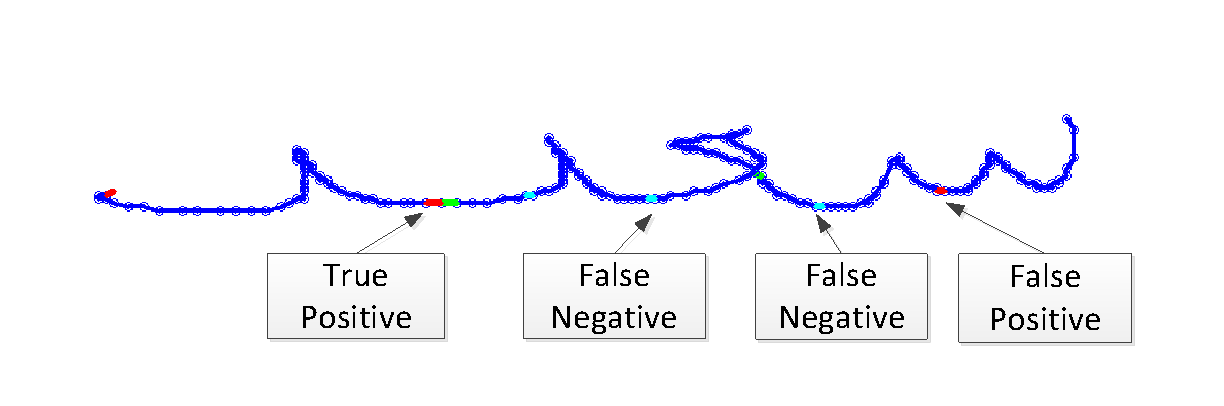
\includegraphics[width=0.9\textwidth]{./figures/sp_types}
\caption{SPs types.}
\label{fig:sp_types}
\end{figure}


%\bibliographystyle{plainnat}
%\bibliography{references}
%
%\end{document}
